% Gradient Info

\tikzset {_cb29xqt9q/.code = {\pgfsetadditionalshadetransform{ \pgftransformshift{\pgfpoint{0 bp } { 0 bp }  }  \pgftransformrotate{-90 }  \pgftransformscale{2 }  }}}
\pgfdeclarehorizontalshading{_xqd1d5nx2}{150bp}{rgb(0bp)=(0.49,0.83,0.13);
rgb(37.5bp)=(0.49,0.83,0.13);
rgb(62.5bp)=(1,1,1);
rgb(100bp)=(1,1,1)}
\tikzset{every picture/.style={line width=0.75pt}} %set default line width to 0.75pt

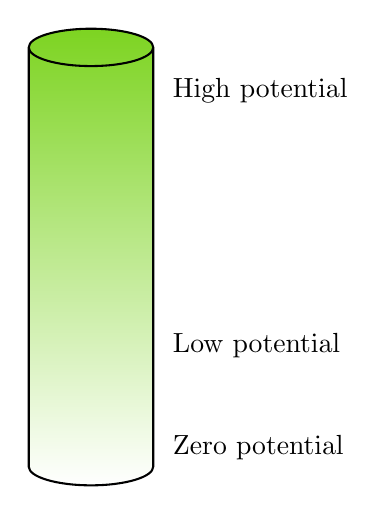
\begin{tikzpicture}[x=0.75pt,y=0.75pt,yscale=-1,xscale=1]
%uncomment if require: \path (0,300); %set diagram left start at 0, and has height of 300

%Shape: Can [id:dp4097434097565138]
    \path  [shading=_xqd1d5nx2,_cb29xqt9q] (497,47.6) -- (497,249.6) .. controls (497,254.57) and (483.57,258.6) .. (467,258.6) .. controls (450.43,258.6) and (437,254.57) .. (437,249.6) -- (437,47.6) .. controls (437,42.63) and (450.43,38.6) .. (467,38.6) .. controls (483.57,38.6) and (497,42.63) .. (497,47.6) .. controls (497,52.57) and (483.57,56.6) .. (467,56.6) .. controls (450.43,56.6) and (437,52.57) .. (437,47.6) ; % for fading
    \draw   (497,47.6) -- (497,249.6) .. controls (497,254.57) and (483.57,258.6) .. (467,258.6) .. controls (450.43,258.6) and (437,254.57) .. (437,249.6) -- (437,47.6) .. controls (437,42.63) and (450.43,38.6) .. (467,38.6) .. controls (483.57,38.6) and (497,42.63) .. (497,47.6) .. controls (497,52.57) and (483.57,56.6) .. (467,56.6) .. controls (450.43,56.6) and (437,52.57) .. (437,47.6) ; % for border


% Text Node
    \draw (505,61) node [anchor=north west][inner sep=0.75pt]   [align=left] {High potential};
% Text Node
    \draw (505,184) node [anchor=north west][inner sep=0.75pt]   [align=left] {Low potential};
% Text Node
    \draw (505,233) node [anchor=north west][inner sep=0.75pt]   [align=left] {Zero potential};


\end{tikzpicture}